\chapter{Evaluation}
\label{ch:evaluation}


\section{Statistics}
\label{sec:statistics}

The statistical evaluation focused both at the extrinsic properties of the application and the development process itself (e.g. code volume, complexity, time spent on development), as well as the intrinsic functional properties of the core functionality that are reflected in the cost of \ac{CPU}-, network-usage and message latency.
Cost of rendering audio and video, as well as general user experience metrics were beyond the scope of the study, as these are highly specific to the task being implemented and are considered transient.

Computers used in the performance evaluation were end-user laptops with the following specifications: \emph{Computer A} is equipped with an 3.1GHz dual-core Intel Core i5 \ac{CPU}, 16GB of \ac{RAM} and a 500GB \ac{SSD}.
\emph{Computer B} is equipped with an Apple M1 Max \ac{CPU} with ten cores, 64GB of \ac{RAM} and a 1TB \ac{SSD}.
Both systems used the Google Chrome browser (version 121.0.6167.85), ran macOS 13.6.3 and connected to the network via 5GHz WiFi.
Both computers used the same \ac{NTP} server to synchronise clocks and the synchronisation was refreshed before each data sampling.

The \emph{latency measurements} were conducted for the data channels and over a consumer 50Mbit \ac{DSL} connection.
They were repeated at different times to account for variance in overall network service quality, and were also conducted over different international \ac{VPN} connections to simulate connection distances within and outside of Europe.
The measurements always used the \ac{BVH} data producer sending the message type for movement qualities alongside 29 key points at a rate of 25 messages per second.
Payload size was 453 bytes for each message, amounting to a required bandwidth of about 11.3 kilobytes per second for each motion capture data stream.
The audio streams were published alongside the data packets, but were not measured for latency.

The results for the latency analysis are shown in separate graphs for each computer containing the datasets for the local and remote messages on each device.

\begin{figure}[h]
\centering
\includegraphics[scale=0.4]{04_Artefakte/01_Abbildungen/latency-computer-a}
\caption[Message latency on Computer A]{Computer A: Latency in milliseconds for local and remote messages\protect}
\label{fig:latencyComputerA}
\end{figure}

Results for computer A (\ref{fig:latencyComputerA}) show a median latency of 18ms for remote messages received over the WebRTC connection and 2ms for the connection from the local data producer to the browser.
Both values show a jitter at a variance of about 11ms for the remote connection and about 6ms for the local connection.

\begin{figure}[h]
\centering
\includegraphics[scale=0.4]{04_Artefakte/01_Abbildungen/latency-computer-b}
\caption[Message latency on Computer B]{Computer B: Latency in milliseconds for local and remote messages\protect}
\label{fig:latencyComputerB}
\end{figure}

The results gathered on computer B (\ref{fig:latencyComputerB}) show a median latency of 48ms for the remote messages and 1ms for the local data producer connection.
Here, the jitter happens at a variance of about 13ms for the remote connection and about 3ms for the local connection.

The development process evaluation was based off the timesheets that were kept during the development process. All recorded tasks were categorised by the language used (e.g. JavaScript), the component worked on and the type of work

\begin{figure}[h]
\centering
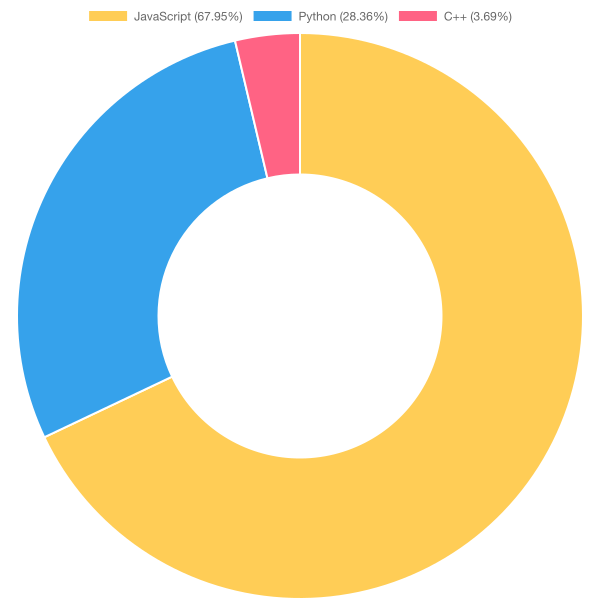
\includegraphics[scale=0.5]{04_Artefakte/01_Abbildungen/time-spent-on-languages}
\caption[Time spent on languages]{Time spent on various programming languages\protect}
\label{fig:timeSpentLanguages}
\end{figure}

\begin{figure}[h]
\centering
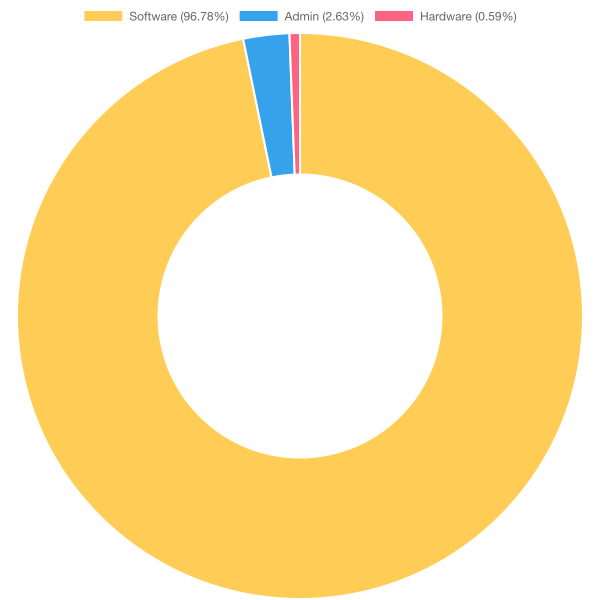
\includegraphics[scale=0.5]{04_Artefakte/01_Abbildungen/time-spent-on-types-of-work}
\caption[Time spent on areas of work]{Time spent on areas of work\protect}
\label{fig:timeSpentTypeOfWork}
\end{figure}

\begin{figure}[h]
\centering
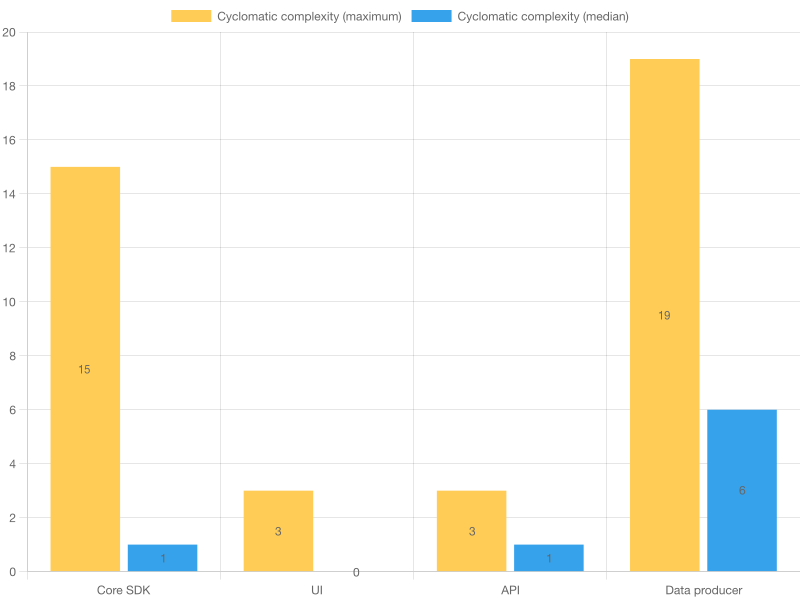
\includegraphics[scale=0.5]{04_Artefakte/01_Abbildungen/code-stats-complexity}
\caption[Cyclomatic complexity]{Cyclomatic complexity per component\protect}
\label{fig:cyclomaticComplexity}
\end{figure}

\begin{figure}[h]
\centering
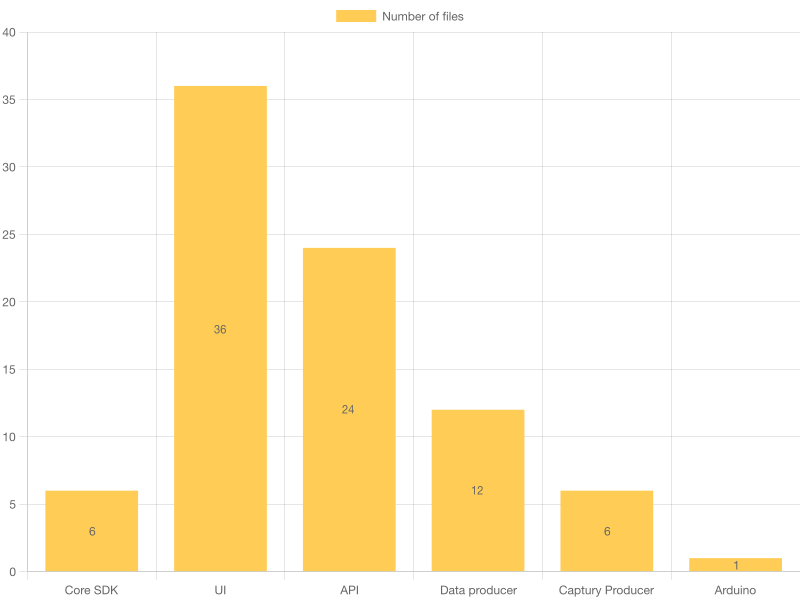
\includegraphics[scale=0.5]{04_Artefakte/01_Abbildungen/code-stats-filecount}
\caption[File count]{Number of source files per application component\protect}
\label{fig:fileCount}
\end{figure}

\begin{figure}[h]
\centering
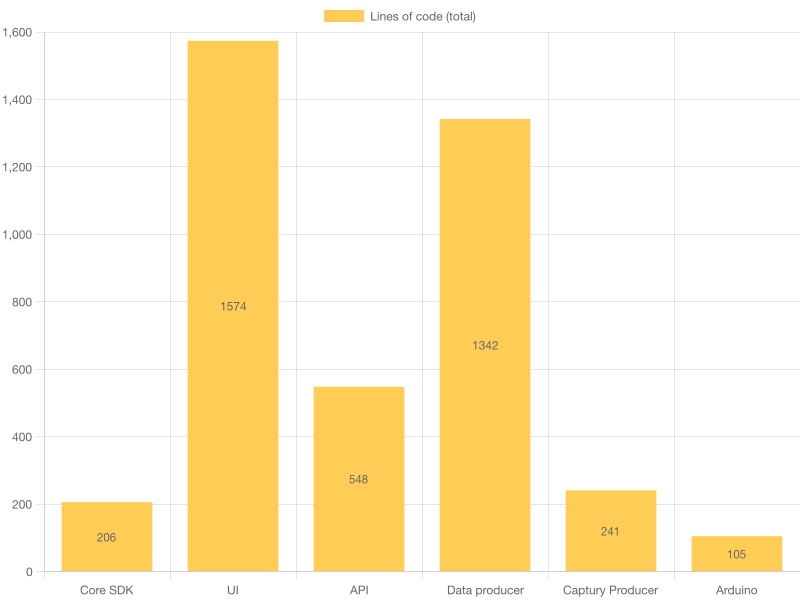
\includegraphics[scale=0.5]{04_Artefakte/01_Abbildungen/code-stats-loc-total}
\caption[Lines of code (total)]{Total lines of code per application component\protect}
\label{fig:linesOfCodeTotal}
\end{figure}

\begin{figure}[h]
\centering
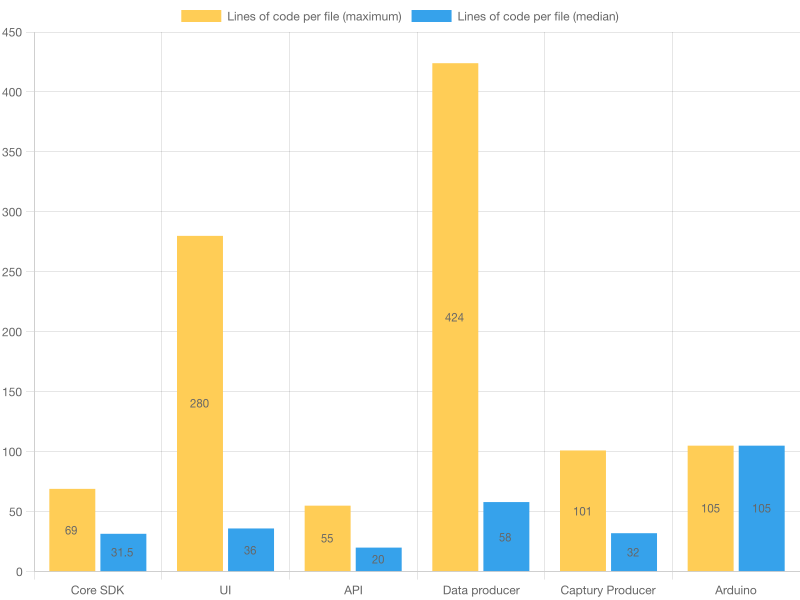
\includegraphics[scale=0.5]{04_Artefakte/01_Abbildungen/code-stats-loc}
\caption[Lines of code]{Maximum and median number of lines of code per application component\protect}
\label{fig:linesOfCode}
\end{figure}

\section{Critical reflection}
\label{sec:critical-reflection}

The development process was carried out in two main timeframes (X and Y) and followed the guiding principles decided in the concept.
It was a mostly pleasant experience with the selected frameworks delivering on their promised functionality and ease of use.
The initial setup was extremely quick due to the ease of setup of the WebRTC server and the quick generation of boilerplate code for the \ac{API} and the \ac{UI}.
However, the web audio standard implementation leaves a lot to desire, especially the support for spatial audio in the browser.
Currently, there is no built-in way to load custom \ac{HRTF} data, which should drastically improve the accuracy of spatial positioning for sound.
There are approaches using a custom build of the Chromium browser~\parencite{chromiumCustomHrtf} or a custom audio node~\parencite{customHrtfAudioNode} which unfortunately does not work with the \ac{SOFA} file format, so it is generally rather disappointing not seeing this thoroughly implemented in the general standard \ac{API}.

The initial setup for the data producers was also relatively quick, due to the large number of examples for the DepthAI \ac{SDK} and the clarity and hands-on approach to the main Python documentation.
The only thing lacking here, was a straightforward way to manage dependencies, as there were different results for the same dependencies being installed via PIP or Conda.

